\documentclass{article}
\usepackage[utf8]{inputenc}
\usepackage[spanish]{babel}
\usepackage{natbib}
\usepackage{graphicx}
\usepackage{mathtools}
\usepackage{color}
\usepackage{soul}
\usepackage{float}
\usepackage{fancyhdr}
\usepackage{adjustbox}
\usepackage{comment}


\pagestyle{fancy}
\lhead{Grupo 4 - Turno 7}
\chead{Trabajo Practico Nro 3}
\rhead{Primer Cuatrimestre 2015}

\begin{document}

\section{Introducción}

En la electrostática elemental se calcula la capacidad de un condensador
plano despreciando los efectos de borde, es decir, suponiendo que las 
líneas de campo se encuentran confinadas entre las placas del mismo. 
Además, se supone que el campo es uniforme y sus líneas son rectas, como se 
ha visto en las clases teóricas y prácticas. En este modelo, si A es 
el área de cada placa, d la separación entre ellas y $ \varepsilon\ $la permitividad del dieléctrico, la capacidad del capacitor plano está dada por $C = \varepsilon\frac{A}{d}$

\section{Objetivos}

En esta experiencia se quiere determinar la variación de la capacidad de 
un condensador de placas paralelas circulares con la separación entre las 
placas como dato. Se compararán para ello los valores experimentales con los 
obtenidos teóricamente a través de distintos modelos. Además, se resolverá numéricamente el problema de un capacitor 
con las características indicadas. Por otro lado, se determinará la 
influencia de la geometría y del instrumento de medición en los resultados 
obtenidos. \\
Para determinar la variación de la 
capacidad de un capacitor de aluminio de placas circulares de radio $R=10 
cm$ y espesor $\delta =6 mm$ se dispone de un electrómetro con 4 rangos de 
voltaje (3V, 10V, 30 V y 100V) y una fuente de tensión variable de 0V a 
30V.

\section{Materiales}

Para realizar la experiencia se utilizaron los siguientes materiales:
\begin{itemize}
	\item Electrómetro
    \item Fuente de tensión variable
    \item Capacitor de aluminio de placas circulares
\end{itemize}
    
    \begin{table}[H]
    \centering
    \begin{tabular}{|l|l|l|}
        \hline
         Radio de las placas	&R(m)	&0,1\\ \hline
         Espesor de placas	&$\delta$(m)	&0,006\\
         \hline
    \end{tabular}
    \caption{Datos del capacitor usado}
    \end{table}
    
\section{Desarrollo}

Se carga el capacitor (con las placas separadas una cierta distancia d) con 
una fuente de corriente continua. Una vez cargado, se mide la 
diferencia de potencial entre sus placas para esa distancia. Luego se modifica la separación 
entre las mismas y se determina la nueva diferencia de potencial. Procedemos así a realizar todas las mediciones para todas las diferentes distancias.\\
Una vez tomadas las mediciones en el laboratorio, calculamos la capacidad del condensador de tres formas diferentes, explicadas en el enunciado del trabajo. Se hicieron los cálculos con el modelo elemental, con corrección por finitud de placas y con corrección por finitud y espesor de placas.\\
Para corroborar los valores obtenidos, se realizó el Problema 5 del enunciado con los mismos valores para la distancia entre placas que los medidos y se calculó el error relativo porcentual entre los valores experimentales y teóricos.\\
Finalmente se calculó la energía almacenada en el capacitor para cada distancia y se obtuvieron conclusiones de todo el trabajo.


\section{Mediciones}
Las mediciones expuestas en la siguiente tabla son aquellas tomadas en el laboratorio.

    \begin{table}[H]
	\centering
	%%%%%%%%%%%%%%%%%%%%%%%%%%%%%%%%%%%%%%%%%%%%%%%%%%%%%%%%%%%%%%%%%%%%%%
%%                                                                  %%
%%  This is a LaTeX2e table fragment exported from Gnumeric.        %%
%%                                                                  %%
%%%%%%%%%%%%%%%%%%%%%%%%%%%%%%%%%%%%%%%%%%%%%%%%%%%%%%%%%%%%%%%%%%%%%%
\begin{tabular}{| c | c | c | c |}
\hline
 & \multicolumn{3}{|c|}{Voltaje (V)} \\ \cline{2-4}
Distancia (mm)	& $1^a$ Medición	&$2^a$ Medición	& $3^a$ Medición\\ \hline
3	&4.4	&4.4	&3.8\\
4	&4.8	&4.8	& 4.2\\
5	&5.3	&5	    &4.4\\
6	&5.6	&5.3	&4.6\\
7	&6	    &5.6	&4.8\\
8	&6.2	&5.8	&5\\
9	&6.4	&6	    &5.1\\
10	&6.4	&6	    &5.2\\
11	&6.6	&6.1	&5.2\\
12	&6.8	&6.2	&5.4\\
13	&6.8	&6.3	&5.6\\
14	&6.8	&6.4	&5.6\\
15	&6.8	&6.4	&5.6\\
16	&6.9	&6.4	&5.6\\
17	&7.2	&6.4	&5.6\\
18	&7.2	&6.5	&5.6\\
19	&7.2	&6.6	&5.7\\
20	&x	    &x	    &5.7\\
25	&x	    &x	    &5.9\\
30	&7.4	&6.8	&6\\
35	&x	    &6.8	&6\\
40	&x	    &x	    &6\\
45	&x	    &x	    &6\\
50	&x	    &x	    &6\\ \hline
\end{tabular}
    \end{table}
    
Para comenzar, elaboramos el siguiente gráfico que muestra las sucesivas diferencias de potencial por las que pasamos al modificar la distancia entre placas.

    \begin{figure}[H]
    \centering
    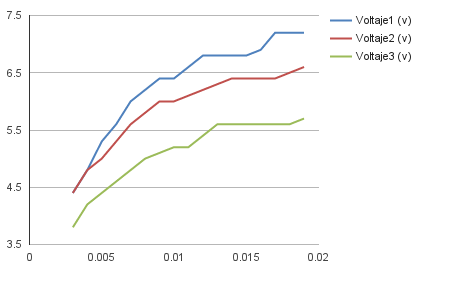
\includegraphics[scale=0.75]{voltajes.png}
    \caption{Gráfico de diferencia de potencial en función de la distancia d(m)}
    \label{fig: 2}
    \end{figure}
    
\section{Resultados Experimentales}

\subsection{Cálculo de la capacidad}
Primeramente, calculamos la capacidad del capacitor los efectos de borde, suponiendo al campo eléctrico como uniforme (por considerar a las 
placas planas infinitas) y confinado en el espacio del dieléctrico. Además es despreciado el espesor de las placas. En este modelo la capacidad está dada por:

\begin{equation}
C_0 = \varepsilon\frac{A}{d} = \varepsilon\frac{\pi R^2}{d}
\end{equation}

Donde $\varepsilon = \varepsilon_0 \varepsilon_r$, R es el radio de las placas y d a 
distancia entre ellas.


A partir del modelo teórico de Kirchhoff, que incluye correcciones en la capacidad debidas a la finitud de las
placas y el espesor de las mismas, se desprende que la capacidad con la corrección debida sólo a la finitud
de las placas está dada por

\begin{equation}
C^{*} = \varepsilon R \bigg[ \pi\frac{R}{d} - 1 + \ln{\bigg(16\pi\frac{R}{d}}\bigg) \bigg]
\end{equation}

El mencionado modelo de Kirchhoff, que incluye las  correcciones debidas a la finitud de las placas y el espesor de las mismas, la capacidad está dada por

\begin{equation} \label{eq:cdelta}
C^{\delta} = \varepsilon \bigg[\pi\frac{R^2}{d} - R + \frac{4 \pi R \delta \ln{\big( 1 + \frac{d}{\delta}\big)}}{d} + R\ln{\bigg(16\pi R\bigg(\frac{1 + \frac{\delta}{d}}{d}}\bigg)\bigg) \bigg]
\end{equation}

Donde es el $\delta$ espesor de las placas.\\

De estas tres formas calculamos la capacidad del condensador para todas las variaciones de la distancia entre placas.

    \begin{table}[H]
	\centering
	%%%%%%%%%%%%%%%%%%%%%%%%%%%%%%%%%%%%%%%%%%%%%%%%%%%%%%%%%%%%%%%%%%%%%%
%%                                                                  %%
%%  This is a LaTeX2e table fragment exported from Gnumeric.        %%
%%                                                                  %%
%%%%%%%%%%%%%%%%%%%%%%%%%%%%%%%%%%%%%%%%%%%%%%%%%%%%%%%%%%%%%%%%%%%%%%
    \begin{adjustbox}{max width=\columnwidth}
    \begin{tabular}{|c|c|c|c|c|}
        \hline
d (mm)	&d (m)	&$C_0$ (pF)	&$C^{*}$ (pF)	&$C^{\delta}$ (pF)\\\hline
3	&0.003	&92.68	&98.36	&108.35\\
4	&0.004	&69.51	&74.94	&84.27\\
5	&0.005	&55.61	&60.84	&69.63\\
6	&0.006	&46.34	&51.41	&59.73\\
7	&0.007	&39.72	&44.65	&52.57\\
8	&0.008	&34.75	&39.57	&47.13\\
9	&0.009	&30.89	&35.61	&42.85\\
10	&0.010	&27.80	&32.42	&39.38\\
11	&0.011	&25.28	&29.81	&36.51\\
12	&0.012	&23.17	&27.63	&34.10\\
13	&0.013	&21.39	&25.77	&32.03\\
14	&0.014	&19.86	&24.18	&30.24\\
15	&0.015	&18.54	&22.80	&28.67\\
16	&0.016	&17.38	&21.58	&27.28\\
17	&0.017	&16.35	&20.50	&26.05\\
18	&0.018	&15.45	&19.55	&24.94\\
19	&0.019	&14.63	&18.68	&23.94\\
20	&0.020	&13.90	&17.91	&23.03\\
25	&0.025	&11.12	&14.93	&19.50\\
30	&0.030	&9.27	&12.92	&17.06\\
35	&0.035	&7.94	&11.45	&15.26\\
40	&0.040	&6.95	&10.34	&13.87\\
45	&0.045	&6.18	&9.47	&12.75\\
50	&0.050	&5.56	&8.76	&11.84\\
    \hline
    \end{tabular}
    \end{adjustbox}
    \end{table}

A continuación graficamos las diversas capacidades en función de la distancia entre placas.

    \begin{figure}[H]
    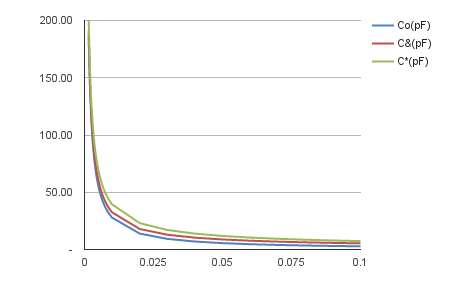
\includegraphics[scale=0.75]{problema5.png}
    \caption{Gráfico de capacidades en función de la distancia d(m)}
    \label{fig:1}
    \end{figure}

\begin{comment}
El cuadro volado
    \begin{table}[H]
    \begin{adjustbox}{max width=\columnwidth}
    \begin{tabular}{|l|l|l|l|l|l|l|l|l|}
        \hline
        Distancia (m)  & Co(pF) & C(pF) & C*(pF) & F & F* & Co(d)/Co(5mm) & C(d)/C(5mm) & C*(d)/C*(5mm)\\ \hline
       0,0015	&185,35	&191,65	&203	&1,034	&1,095	&3,33	&3,15	&2,916\\
0,002	&139,02	&145,06	&155,88	&1,043	&1,121	&2,5	&2,384	&2,239\\
0,0025	&111,21	&117,06	&127,44	&1,053	&1,146	&2	&1,924	&1,83\\
0,003	&92,68	&98,36	&108,35	&1,061	&1,169	&1,67	&1,617	&1,556\\
0,0035	&79,44	&84,99	&94,63	&1,07	&1,191	&1,43	&1,397	&1,359\\
0,004	&69,51	&74,94	&84,27	&1,078	&1,212	&1,25	&1,232	&1,21\\
0,0045	&61,78	&67,11	&76,16	&1,086	&1,233	&1,11	&1,103	&1,094\\
0,005	&55,61	&60,84	&69,63	&1,094	&1,252	&1	&1	&1\\
0,0055	&50,55	&55,7	&64,25	&1,102	&1,271	&0,91	&0,916	&0,923\\
0,006	&46,34	&51,41	&59,73	&1,109	&1,289	&0,83	&0,845	&0,858\\
0,0065	&42,77	&47,77	&55,89	&1,117	&1,307	&0,77	&0,785	&0,803\\
0,007	&39,72	&44,65	&52,57	&1,124	&1,324	&0,71	&0,734	&0,755\\
0,0075	&37,07	&41,95	&49,68	&1,131	&1,34	&0,67	&0,689	&0,714\\
0,008	&34,75	&39,57	&47,13	&1,139	&1,356	&0,62	&0,65	&0,677\\
0,0085	&32,71	&37,47	&44,87	&1,146	&1,372	&0,59	&0,616	&0,644\\
0,009	&30,89	&35,61	&42,85	&1,153	&1,387	&0,56	&0,585	&0,615\\
0,0095	&29,27	&33,93	&41,03	&1,159	&1,402	&0,53	&0,558	&0,589\\
0,01	&27,8	&32,42	&39,38	&1,166	&1,417	&0,5	&0,533	&0,566\\
0,02	&13,9	&17,91	&23,03	&1,288	&1,657	&0,25	&0,294	&0,331\\
0,03	&9,27	&12,92	&17,06	&1,394	&1,841	&0,17	&0,212	&0,245\\
0,04	&6,95	&10,34	&13,87	&1,488	&1,995	&0,12	&0,17	&0,199\\
0,05	&5,56	&8,76	&11,84	&1,575	&2,129	&0,1	&0,144	&0,17\\
0,06	&4,63	&7,67	&10,42	&1,655	&2,248	&0,08	&0,126	&0,15\\
0,07	&3,97	&6,87	&9,36	&1,73	&2,357	&0,07	&0,113	&0,134\\
0,08	&3,48	&6,25	&8,54	&1,8	&2,457	&0,06	&0,103	&0,123\\
0,09	&3,09	&5,76	&7,88	&1,866	&2,55	&0,06	&0,095	&0,113\\
0,1	&2,78	&5,36	&7,33	&1,929	&2,636	&0,05	&0,088	&0,105\\
    \hline
    \end{tabular}
    \end{adjustbox}
    \end{table}
\end{comment}

    
\subsection{Comparación de capacidades con valores teóricos}
Para corroborar las capacidades calculadas a partir de las mediciones del laboratorio, solucionamos el Problema 5 del 
enunciado del trabajo para los mismos valores de la distancia d. En el siguiente cuadro se encuentran los resultados del 
problema junto a nuestros valores experimentales y sus respectivos errores porcentuales.


   \begin{table}[H]
   \centering
   \begin{adjustbox}{max width=\columnwidth}
   \begin{tabular}{|c|c|c|c|c|}
    	\hline
        d (mm) & d (m) & Capacidad experimental(pF) & Capacidad teórica (pF) & $\varepsilon$ de capacidad \\ \hline
3	&0,003	&92,68	& 92,68    	&0,00\\
4	&0,004	&69,51	& 69,51    	&0,00\\
5	&0,005	&55,61	& 55,61    	&0,00\\
6	&0,006	&46,34	& 46,34    	&0,00\\
7	&0,007	&39,72	& 39,72    	&0,00\\
8	&0,008	&34,75	& 34,75    	&0,00\\
9	&0,009	&30,89	& 30,89    	&0,00\\
10	&0,01	&27,80	& 27,80    	&0,00\\
11	&0,011	&25,28	& 25,28    	&0,00\\
12	&0,012	&23,17	& 23,17    	&0,00\\
13	&0,013	&21,39	& 21,39    	&0,00\\
14	&0,014	&19,86	& 19,86    	&0,00\\
15	&0,015	&18,54	& 18,54    	&0,00\\
16	&0,016	&17,38	& 17,38    	&0,00\\
17	&0,017	&16,35	& 16,35    	&0,00\\
18	&0,018	&15,45	& 15,45    	&0,00\\
19	&0,019	&14,63	& 14,63    	&0,00\\
20	&0,02	&13,90	& 13,90    	&0,00\\
25	&0,025	&11,12	& 11,12    	&0,00\\
30	&0,03	&9,27	& 9,27    	&0,00\\
35	&0,035	&7,94	& 7,94    	&0,00\\
40	&0,04	&6,95	& 6,95    	&0,00\\
45	&0,045	&6,18	& 6,18    	&0,00\\
50	&0,05	&5,56	& 5,56    	&0,00\\
    \hline
	\end{tabular}
	\end{adjustbox}
	\caption{Tabla comparativa de $C_0$ (pF)}
    \end{table}


   \begin{table}[H]
   \centering
   \begin{adjustbox}{max width=\columnwidth}
   \begin{tabular}{|c|c|c|c|c|}
    	\hline
        d (mm) & d (m) & Capacidad experimental(pF) & Capacidad teórica (pF) & $\varepsilon$ de capacidad \\ \hline
3	&0,003	&108,35	& 108,00    	&0,33\\
4	&0,004	&84,27	& 83,82    	&0,53\\
5	&0,005	&69,63	& 69,09    	&0,77\\
6	&0,006	&59,73	& 59,12    	&1,02\\
7	&0,007	&52,57	& 51,90    	&1,29\\
8	&0,008	&47,13	& 46,39    	&1,57\\
9	&0,009	&42,85	& 42,05    	&1,86\\
10	&0,01	&39,38	& 38,53    	&2,17\\
11	&0,011	&36,51	& 35,61    	&2,48\\
12	&0,012	&34,10	& 33,14    	&2,79\\
13	&0,013	&32,03	& 31,03    	&3,11\\
14	&0,014	&30,24	& 29,20    	&3,43\\
15	&0,015	&28,67	& 27,59    	&3,75\\
16	&0,016	&27,28	& 26,17    	&4,08\\
17	&0,017	&26,05	& 24,90    	&4,41\\
18	&0,018	&24,94	& 23,76    	&4,73\\
19	&0,019	&23,94	& 22,73    	&5,06\\
20	&0,02	&23,03	& 21,79    	&5,39\\
25	&0,025	&19,50	& 18,14    	&7,00\\
30	&0,03	&17,06	& 15,60    	&8,57\\
35	&0,035	&15,26	& 13,72    	&10,07\\
40	&0,04	&13,87	& 12,27    	&11,49\\
45	&0,045	&12,75	& 11,11    	&12,83\\
50	&0,05	&11,84	& 10,17    	&14,10\\
    \hline
	\end{tabular}
	\end{adjustbox}
	\caption{Tabla comparativa de $C^{*}$ (pF)}
    \end{table}



   \begin{table}[H]
   \centering
   \begin{adjustbox}{max width=\columnwidth}
   \begin{tabular}{|c|c|c|c|c|}
    	\hline
        d (mm) & d (m) & Capacidad experimental(pF) & Capacidad teórica (pF) & $\varepsilon$ de capacidad \\ \hline
3	&0,003	&98,36	& 98,36    	&0,00\\
4	&0,004	&74,94	& 74,94    	&0,00\\
5	&0,005	&60,84	& 60,84    	&0,00\\
6	&0,006	&51,41	& 51,41    	&0,00\\
7	&0,007	&44,65	& 44,65    	&0,00\\
8	&0,008	&39,57	& 39,57    	&0,00\\
9	&0,009	&35,61	& 35,61    	&0,00\\
10	&0,01	&32,42	& 32,42    	&0,00\\
11	&0,011	&29,81	& 29,81    	&0,00\\
12	&0,012	&27,63	& 27,63    	&0,00\\
13	&0,013	&25,77	& 25,77    	&0,00\\
14	&0,014	&24,18	& 24,18    	&0,00\\
15	&0,015	&22,80	& 22,80    	&0,00\\
16	&0,016	&21,58	& 21,58    	&0,00\\
17	&0,017	&20,50	& 20,50    	&0,00\\
18	&0,018	&19,55	& 19,55    	&0,00\\
19	&0,019	&18,68	& 18,68    	&0,00\\
20	&0,02	&17,91	& 17,91    	&0,00\\
25	&0,025	&14,93	& 14,93    	&0,00\\
30	&0,03	&12,92	& 12,92    	&0,00\\
35	&0,035	&11,45	& 11,45    	&0,00\\
40	&0,04	&10,34	& 10,34    	&0,00\\
45	&0,045	&9,47	& 9,47    	&0,00\\
50	&0,05	&8,76	& 8,76    	&0,00\\
    \hline
	\end{tabular}
	\end{adjustbox}
	\caption{Tabla comparativa de $C^{\delta}$ (pF)}
    \end{table}




    
\subsection{Cálculo de energía almacenada en el capacitor}

Para el calculo de la energia almacenada en el capacitor se utilizó la siguiente formula:

\begin{equation}
    E = \frac{C^{\delta} \Delta V^{2}}{2} 
\end{equation}

Donde $C^{\delta}$ corresponde a la ecuacion \ref{eq:cdelta} y $\Delta V$ a las diferencias de potencial medidas en 
el laboratorio.

    
    \begin{table}[H]
	\centering
    %%%%%%%%%%%%%%%%%%%%%%%%%%%%%%%%%%%%%%%%%%%%%%%%%%%%%%%%%%%%%%%%%%%%%%
%%                                                                  %%
%%  This is a LaTeX2e table fragment exported from Gnumeric.        %%
%%                                                                  %%
%%%%%%%%%%%%%%%%%%%%%%%%%%%%%%%%%%%%%%%%%%%%%%%%%%%%%%%%%%%%%%%%%%%%%%
%%%%%%%%%%%%%%%%%%%%%%%%%%%%%%%%%%%%%%%%%%%%%%%%%%%%%%%%%%%%%%%%%%%%%%
\begin{tabular}{| l | c | r |}
\hline
Distancia (mm)	&Voltaje (V)	&Energía (J)\\ \hline
3	&3.8	&8.61E-10\\
4	&4.2	&1.05E-09\\
5	&4.4	&1.15E-09\\
6	&4.6	&1.26E-09\\
7	&4.8	&1.37E-09\\
8	&5	    &1.49E-09\\
9	&5.1	&1.55E-09\\
10	&5.2	&1.61E-09\\
11	&5.2	&1.61E-09\\
12	&5.4	&1.74E-09\\
13	&5.6	&1.87E-09\\
14	&5.6	&1.87E-09\\
15	&5.6	&1.87E-09\\
16	&5.6	&1.87E-09\\
17	&5.6	&1.87E-09\\
18	&5.6	&1.87E-09\\
19	&5.7	&1.94E-09\\
20	&5.7	&1.94E-09\\
25	&5.9	&2.08E-09\\
30	&6	    &2.15E-09\\
35	&6	    &2.15E-09\\
40	&6	    &2.15E-09\\
45	&6	    &2.15E-09\\
50	&6	    &2.15E-09\\ \hline
\end{tabular}
    \caption{Energia (J) en funcion de la distancia entre placas (mm)}
    \label{table:energiaEnCapacitor}
    \end{table}

    Con estos valores graficamos la energía del capacitor en función de la distancia entre placas.
   
    \begin{figure}[H]
    \centering
    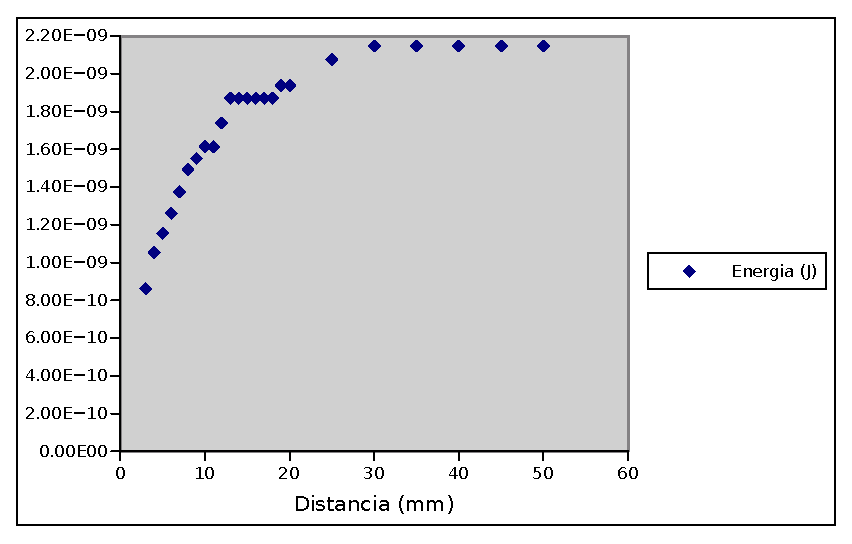
\includegraphics[scale=0.67]{energia_en_capacitor.eps}
    \caption{Energia (J) en función de la distancia entre placas (mm)}
    \label{fig:energiaEnCapacitorGrafico}
    \end{figure}

    Mediante el cuadro \ref{table:energiaEnCapacitor} y el gráfico \ref{fig:energiaEnCapacitorGrafico}, es posible apreciar que la energía almacenada en el capacitor aumenta a medida que la separación entre las placas conductoras se incrementa. Otro aspecto interesante es que la función de la energía converge en un valor cercano a $2.15E-09 J$, esto coincide con la convergencia de la diferencia de potencial y la capacidad en función de la distancia. A partir de este resultado, se puede determinar que la energía almacenada en el condensador no continuara aumentando a pesar de que se siga incrementando la distancia de separación entre placas. 

\section{Conclusiones}
\begin{itemize}
	
	\item La toma de datos provenientes de la experiencia está claramente condicionada por 
	el aparato de medición y los operadores. Se pierde precisión.
    
    \item Se observó que en la tercera medición todos los valores obtenidos habían 
    disminuido respecto a las primeras dos mediciones; la disminución va entre un 12\% y un 
    20\%. Esta situación es de interés y por lo tanto se procedió a analizarla. Llegamos a 
    la conclusión de que esto se debe a que, a lo largo de la experiencia, el capacitor va 
    perdiendo carga.    
    
    \item Entre 10mm y 20mm de distancia, la energía del capacitor se mantiene casi 
    constante, al igual que entre los 30 y 50 milímetros.
    
    \item En el cálculo de capacidades, nos encontramos con error nulo en la etapa donde se 
    desprecia espesor de las placas y efectos de borde. Cuando se procede a usar el modelo 
    teórico de Kirchhoff, teniendo en cuenta la finitud de las placas, los errores aumentan y se mantienen entre un 0,3\% y 14\% de diferencia. A pesar de que esperábamos que los valores de la tercer forma de cálculo presentaran aún más error respecto a los valores experimentales, obtuvimos un error nulo.
    
\end{itemize}


\end{document}